\section{Date: 2026-11-21}
\noindent \textbf{Series ID: MESTAMUSERGSP} 

\noindent This series is titled Real Gross Domestic Product: Amusement, Gambling, and Recreation Industries (713) in the Mideast BEA Region and has a frequency of Annual. The units are Millions of Chained 2017 Dollars and the seasonal adjustment is Not Seasonally Adjusted.The observation start date is 1997-01-01 and the observation end date is 2025-01-01.The popularity of this series is 1. \\ 

\noindent \textbf{Series ID: BCEMFT02ZAQ460S} 

\noindent This series is titled Business Tendency Surveys: Employment: Economic Activity: Construction: Future Tendency for South Africa and has a frequency of Quarterly. The units are Percentage balance and the seasonal adjustment is Seasonally Adjusted.The observation start date is 2001-04-01 and the observation end date is 2026-07-01.The popularity of this series is 1. \\ 

\subsection{Raw Regression}
\noindent Regresses the two series against each other directly. A significant result here can come just as easily from both series sharing a long-run trend as from any real relationship.

\begin{center}
\begin{tabular}{lclc}
\toprule
\textbf{Dep. Variable:}             & value\_fred\_BCEMFT02ZAQ460S & \textbf{  R-squared:         } &     0.092   \\
\textbf{Model:}                     &             OLS              & \textbf{  Adj. R-squared:    } &     0.050   \\
\textbf{Method:}                    &        Least Squares         & \textbf{  F-statistic:       } &     2.218   \\
\textbf{Date:}                      &       Sat, 21 Nov 2026       & \textbf{  Prob (F-statistic):} &    0.151    \\
\textbf{Time:}                      &           18:21:08           & \textbf{  Log-Likelihood:    } &   -104.46   \\
\textbf{No. Observations:}          &                24            & \textbf{  AIC:               } &     212.9   \\
\textbf{Df Residuals:}              &                22            & \textbf{  BIC:               } &     215.3   \\
\textbf{Df Model:}                  &                 1            & \textbf{                     } &             \\
\textbf{Covariance Type:}           &          nonrobust           & \textbf{                     } &             \\
\bottomrule
\end{tabular}
\begin{tabular}{lcccccc}
                                    & \textbf{coef} & \textbf{std err} & \textbf{t} & \textbf{P$> |$t$|$} & \textbf{[0.025} & \textbf{0.975]}  \\
\midrule
\textbf{const}                      &      23.5799  &       23.892     &     0.987  &         0.334        &      -25.970    &       73.129     \\
\textbf{value\_fred\_MESTAMUSERGSP} &      -0.0030  &        0.002     &    -1.489  &         0.151        &       -0.007    &        0.001     \\
\bottomrule
\end{tabular}
\begin{tabular}{lclc}
\textbf{Omnibus:}       &  0.589 & \textbf{  Durbin-Watson:     } &    0.915  \\
\textbf{Prob(Omnibus):} &  0.745 & \textbf{  Jarque-Bera (JB):  } &    0.598  \\
\textbf{Skew:}          & -0.322 & \textbf{  Prob(JB):          } &    0.741  \\
\textbf{Kurtosis:}      &  2.571 & \textbf{  Cond. No.          } & 7.18e+04  \\
\bottomrule
\end{tabular}
%\caption{OLS Regression Results}
\end{center}

Notes: \newline
 [1] Standard Errors assume that the covariance matrix of the errors is correctly specified. \newline
 [2] The condition number is large, 7.18e+04. This might indicate that there are \newline
 strong multicollinearity or other numerical problems.

\begin{figure}
\centering
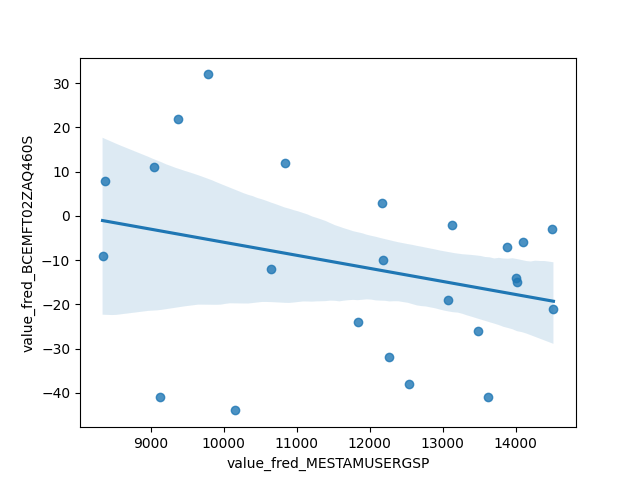
\includegraphics[scale = 0.9]{plots/plot_2026-11-21.png}
\caption{Raw Regression Plot for 2026-11-21}
\end{figure}
\newpage
\subsection{Detrended Regression}
\noindent Regresses the residuals of each series after removing its own linear time trend, so a shared trend can no longer drive the result on its own. A relationship that stays significant here is better evidence of a genuine link between the two series.

\begin{center}
\begin{tabular}{lclc}
\toprule
\textbf{Dep. Variable:}                        & value\_fred\_BCEMFT02ZAQ460S\_detrended & \textbf{  R-squared:         } &     0.038   \\
\textbf{Model:}                                &                   OLS                   & \textbf{  Adj. R-squared:    } &    -0.006   \\
\textbf{Method:}                               &              Least Squares              & \textbf{  F-statistic:       } &    0.8618   \\
\textbf{Date:}                                 &             Sat, 21 Nov 2026            & \textbf{  Prob (F-statistic):} &    0.363    \\
\textbf{Time:}                                 &                 18:21:08                & \textbf{  Log-Likelihood:    } &   -102.01   \\
\textbf{No. Observations:}                     &                      24                 & \textbf{  AIC:               } &     208.0   \\
\textbf{Df Residuals:}                         &                      22                 & \textbf{  BIC:               } &     210.4   \\
\textbf{Df Model:}                             &                       1                 & \textbf{                     } &             \\
\textbf{Covariance Type:}                      &                nonrobust                & \textbf{                     } &             \\
\bottomrule
\end{tabular}
\begin{tabular}{lcccccc}
                                               & \textbf{coef} & \textbf{std err} & \textbf{t} & \textbf{P$> |$t$|$} & \textbf{[0.025} & \textbf{0.975]}  \\
\midrule
\textbf{const}                                 &   -1.213e-12  &        3.618     & -3.35e-13  &         1.000        &       -7.503    &        7.503     \\
\textbf{value\_fred\_MESTAMUSERGSP\_detrended} &       0.0030  &        0.003     &     0.928  &         0.363        &       -0.004    &        0.010     \\
\bottomrule
\end{tabular}
\begin{tabular}{lclc}
\textbf{Omnibus:}       &  0.229 & \textbf{  Durbin-Watson:     } &    0.923  \\
\textbf{Prob(Omnibus):} &  0.892 & \textbf{  Jarque-Bera (JB):  } &    0.392  \\
\textbf{Skew:}          & -0.179 & \textbf{  Prob(JB):          } &    0.822  \\
\textbf{Kurtosis:}      &  2.487 & \textbf{  Cond. No.          } & 1.13e+03  \\
\bottomrule
\end{tabular}
%\caption{OLS Regression Results}
\end{center}

Notes: \newline
 [1] Standard Errors assume that the covariance matrix of the errors is correctly specified. \newline
 [2] The condition number is large, 1.13e+03. This might indicate that there are \newline
 strong multicollinearity or other numerical problems.

\begin{figure}
\centering
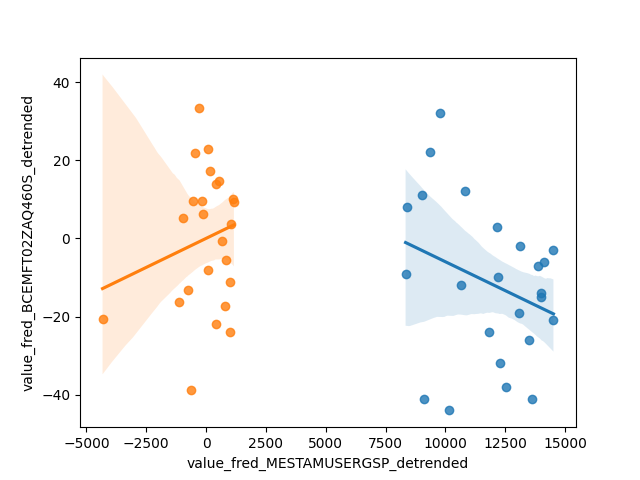
\includegraphics[scale = 0.9]{plots/plot_2026-11-21_detrended.png}
\caption{Detrended Regression Plot for 2026-11-21}
\end{figure}
\newpage
